\subtop{Kreuzungsfreie geradlinige Gitterlayouts}{-1.6}
Jeder planare Graph hat eine kreuzungsfreie, geradlinige Standardrepräsentation. (Nachteil der Konstruktion: hohe Auflösung nötig, weil die Kantenlängen stark variieren können)
%		\vspace*{-1.5\baselineskip}
		\ProofIdea
		\vspace*{-0.5\baselineskip}
		Durch Konstruktion (Funktioniert nicht mit allen Nachbarn, nur bei Knoten mit \textbf{genau} zwei Nachbarn!):\\
		\hspace*{-1cm}\begin{minipage}{0.27\textwidth}
			\usetikzlibrary{positioning,patterns,calc,arrows}

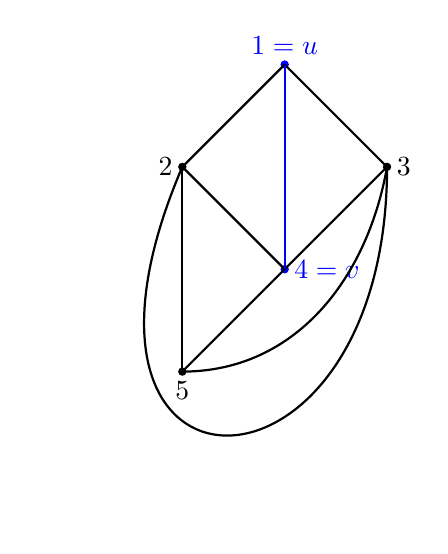
\begin{tikzpicture}[scale=0.65]

\foreach[count=\c] \x/\y/\a in {0/2/90,-2/0/180,2/0/0,0/-2/0,-2/-4/270}{
	\ifnum\c=1{
		\coordinate[label={[color=blue]\a:$\c=u$}](\c) at (\x,\y);
		\draw[fill,color=blue](\c)circle[radius=2pt];
	}\else{
		\ifnum\c=4{
			\coordinate[label={[color=blue]\a:$\c=v$}](\c) at (\x,\y);
			\draw[fill,color=blue](\c)circle[radius=2pt];
		}\else{
			\coordinate[label={\a:$\c$}](\c) at (\x,\y);
			\draw[fill](\c)circle[radius=2pt];
		}\fi
	}\fi
}

\foreach \x/\y in {1/2,1/3,2/5,2/4,3/4,4/5}
	\draw[-,thick](\x)--(\y);

\draw[-,thick](3)to[out=260,in=0](5);
\draw[thick] (2) .. controls (-5,-7) and (2,-7) .. (3);

\draw[-,color=blue,thick](1)to(4);
\end{tikzpicture}
		\end{minipage}
		\hspace*{0.5cm}\begin{minipage}{0.21\textwidth}
			\usetikzlibrary{positioning,patterns,calc,arrows}

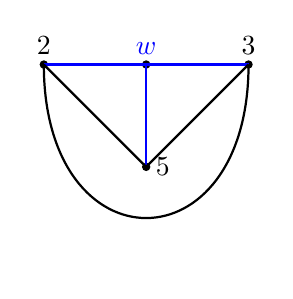
\begin{tikzpicture}[scale=0.65]
\coordinate[label={[color=blue]90:$w$}](w) at (0,0);
\coordinate[label={90:$2$}](2) at (-2,0);
\coordinate[label={90:$3$}](3) at (2,0);
\coordinate[label={0:$5$}](5) at (0,-2);

\foreach \x in {w,2,3,5}{
		\draw[fill](\x)circle[radius=2pt];
}

\foreach \x in {2,3,5}
	\draw[-,thick,color=blue](w)--(\x);
\foreach \x/\y in {2/5,3/5}
	\draw[-,thick](\x)--(\y);
\draw[thick] (2) .. controls (-2,-4) and (2,-4) .. (3);

\end{tikzpicture}
		\end{minipage}
		\hspace*{-0.3cm}\begin{minipage}{0.23\textwidth}
			\usetikzlibrary{positioning,patterns,calc,arrows}

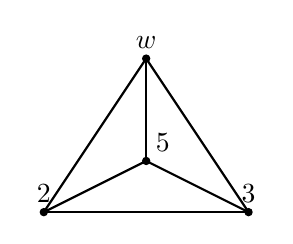
\begin{tikzpicture}[scale=0.65]
\coordinate[label={90:$w$}](w) at (0,0);
\coordinate[label={90:$2$}] (2) at (-2,-3) {};
\coordinate[label={90:$3$}] (3) at (2,-3) {};
\coordinate[label={20:$5$}](5) at (0,-2);
\foreach \x in {w,2,3,5}{
		\draw[fill](\x)circle[radius=2pt];
}

\foreach \x in {2,3,5}
	\draw[-,thick](w)--(\x);
\foreach \x/\y in {2/5,3/5,2/3}
	\draw[-,thick](\x)--(\y);

\end{tikzpicture}
		\end{minipage}
		\begin{minipage}{0.23\textwidth}
			\usetikzlibrary{positioning,patterns,calc,arrows}

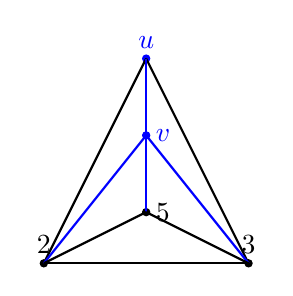
\begin{tikzpicture}[scale=0.65]
\coordinate[label={[color=blue]90:$u$}](u) at (0,0);
\coordinate[label={[color=blue]0:$v$}](v) at (0,-1.5);
\coordinate[label={90:$2$}] (2) at (-2,-4) {} {};
\coordinate[label={90:$3$}] (3) at (2,-4) {} {};
\coordinate[label={0:$5$}] (5) at (0,-3) {};
\foreach \x in {2,3,5}{
		\draw[fill](\x)circle[radius=2pt];
}
\draw[fill,color=blue](u)circle[radius=2pt];
\draw[fill,color=blue](v)circle[radius=2pt];

\foreach \x in {2,3}
	\draw[-,thick](u)--(\x);

\foreach \x in {2,3,u,5}{
	\draw[-,thick,color=blue](v)--(\x);
}
\foreach \x/\y in {2/5,3/5,2/3}
	\draw[-,thick](\x)--(\y);

\end{tikzpicture}
		\end{minipage}
\topbreak
\vspace*{-2\baselineskip}
\subsection{Shift-Methode (Gittergröße $\BigO(n)\times\BigO(n)$)}
\subsubsection{Definitionen:}
\begin{description}[itemsep=-1pt]
	\item[connectivity:] $\kappa(G)$ ist die kleinste Anzahl von Knoten, die entfernt werden müssen, damit $G$ nicht mehr zusammenhängend ist
	\item[maximal planar/trianguliert:] durch Hinzufügen einer Kante, wäre der Graph nicht mehr planar
	\item[kombinatorische Einbettung:] z.B. die kreisförmige Anordnung der Kanten um jeden Knoten des Graphen
	\item[chord:] eine Kante zwischen zwei Knoten $v,w$ auf einem Kreis $C$, wobei $v$ und $w$ auf $C$ nicht nebeneinander liegen
	\item[kanonische Ordnung:] eine Ordnung $\pi=(v_1,\dots,v_n)$, für die für jedes $3\leq k\leq n$ gilt:
		\begin{description}
			\item[co1] Knoten $\{v_1,\dots,v_k\}$ induzieren einen zweifach verbundenen und innen triangulierten Graphen
			\item[co2] $(v_1,v_2)$ ist eine Außenkante von $G_k$
			\item[co3] $k<n\Rightarrow v_{k+1}$ liegt auf der Außenfläche von $G_k$ und alle Nachbarn von $v_{k+1}$ in $G_k$ erscheinen nacheinander auf $C_0(G_k)$
		\end{description}
\end{description}
Jeder triangulierte, planare Graph besitzt eine kanonische Ordnung (durch Konstruktion mit \textbf{co1-3} klar)
\subsubsection{Ablauf}
\begin{enumerate}[itemsep=-1pt]
	\item Hinzufügen von Kanten bis der Graph zweifach zusammenhängend ist
	\item Triangulation durch Hinzufügen weiterer Kanten
	\item Bestimmung einer kanonischen Ordnung der Knoten (\algobreak\algo{kanonische Ordnung}{\begin{algorithm}[H]
	\SetAlgoVlined
	\SetKwProg{Fn}{Function}{}{end}
	\KwIn{triangulierter planarer Graph $G=(V,E)$ mit $C_0(G)=\{v_1,v_2,v_3\} $}
	\KwData{mark($v$)$=$ true, falls $v$ zu $\pi$ hinzugefügt wurde\\out($v$)$=$ true, falls $v\in C_0(G_k)$\\chords($v$)$= \#$ der \textit{chords} von $C_0(G_k)$, dessen Endknoten $v$ ist}
	\KwOut{kanonische Ordnung $\pi=(v_1,v_2,\dots,v_n)$}
	\BlankLine
	\Begin{
		\ForAll{$v\in V$}{
			$chords(v)\leftarrow 0$;\\
			$out(v)\leftarrow $ false; \\
			$mark(v)\leftarrow $ false;
		}
		$out(v_1),out(v_2),out(v_3) \leftarrow$ true;
		\For{$k=3,\dots, 3$}{
			wähle $v\neq v_1,v_2$ mit $mark(v)=$ false, $out(v)=$ false, $chords(v)=0$;\\
			$v_k\leftarrow v$;\\
			$mark(v)\leftarrow$ true;\\
			$(w_1=v_1,w_2,\dots,w_{t-1},w_t=v_2)\leftarrow C_0(G_{k-1})$;\\
			$(w_p,\dots,w_q)\leftarrow$ unmarkierte Nachbarn von $v_k$;\\
			\For{$i=p,\dots,q$}{
				$out(w_i)\leftarrow $ true;\\
				Update der chord-Zähler für $w_i$ und alle seine Nachbarn;
			}
		}
	}
\end{algorithm}}, in Linearzeit)
	\item inkrementelle Bestimmung relativer Koordinaten der Knoten
	\item Bestimmung absoluter Koordinaten
	\item Herausnehmen aller Kanten, die nicht zum Ausgangsgraphen gehören
\end{enumerate}
\subsubsection{Algorithmus}
\begin{itemize}[itemsep=-1pt]
	\item Einfügungsreihenfolge der Knoten entspricht der kanonischen Ordnung
	\item Anfangsknoten $v_1,v_2,v_3$
	\item Einfügen von $v_k$ in das Layout von $G_{k-1}$
	\item zum Sicherstellen der Planarität werden die Knoten zum Teil horizontal verschoben
	\item jeder Knoten hat eine Liste $L(v)$ mit Knoten, die zusammen mit $v$ verschoben werden müssen
\end{itemize}
\vspace*{-\baselineskip}
\usetikzlibrary{positioning,calc,arrows}
\begin{tikzpicture}[node distance=-1.25cm]
\node(1)at(0,0){\usetikzlibrary{positioning,calc,arrows}
\begin{tikzpicture}[every node/.style={draw,circle,fill},node distance=0cm,scale=0.4]

%\draw[color=black!30](-1.5,-1.5)grid(29.5,10.5);

\foreach[count=\c] \x/\y in {0/0,2/2,4/4,6/2,7/3,9/5,10/6,11/5,12/4,13/5,14/6,15/5,16/4,18/2,19/1,20/2,22/4,23/5,25/3,27/1,28/0}
	\node[scale=0.75] (v\c) at (\x,\y) {};

\draw (v1) -- (v2) -- (v3) -- (v4) -- (v5) -- (v6) -- (v7) -- (v8) -- (v9) -- (v10)--(v11) -- (v12) -- (v13) -- (v14) -- (v15) -- (v16) -- (v17) -- (v18) -- (v19) -- (v20) -- (v21)--(v1);

\node[draw=none,fill=none,below=of v1] {\Large$v_1$};
\node[draw=none,fill=none,below=of v21] {\Large$v_2$};

\node[scale=0.75] (vk) at (12,8) {};
\node[draw=none,fill=none,above=of vk,yshift=-0.2cm] {\Large$v_k$};

\def\a{20}

\foreach[count=\c] \x in {5,6,...,14}
	\draw[dashed,color=blue](vk)to[out=160+\c*\a,in=90](v\x);

\draw[very thick,color=red]  plot[smooth, tension=.7] coordinates {(7.5,6) (8,4) (7.5,2) (8,0) (7.5,-2)};
\draw[very thick,color=red]  plot[smooth, tension=.7] coordinates {(17,6) (17.5,4) (17,2) (17.5,0) (17,-2)};

\draw[->,>=latex,line width=3pt,color=red] (17.5,-1) -- (19,-1);
\draw[->,>=latex,line width=3pt,color=red] (17.75,-0.5) -- (19.25,-0.5);

\draw[->,>=latex,line width=3pt,color=red] (7.5,-1) -- (6,-1);
\draw[->,>=latex,line width=3pt,color=red] (7.75,-0.5) -- (6.25,-0.5);
\end{tikzpicture}};
\node[below=of 1,xshift=4cm]{\usetikzlibrary{positioning,calc,arrows}
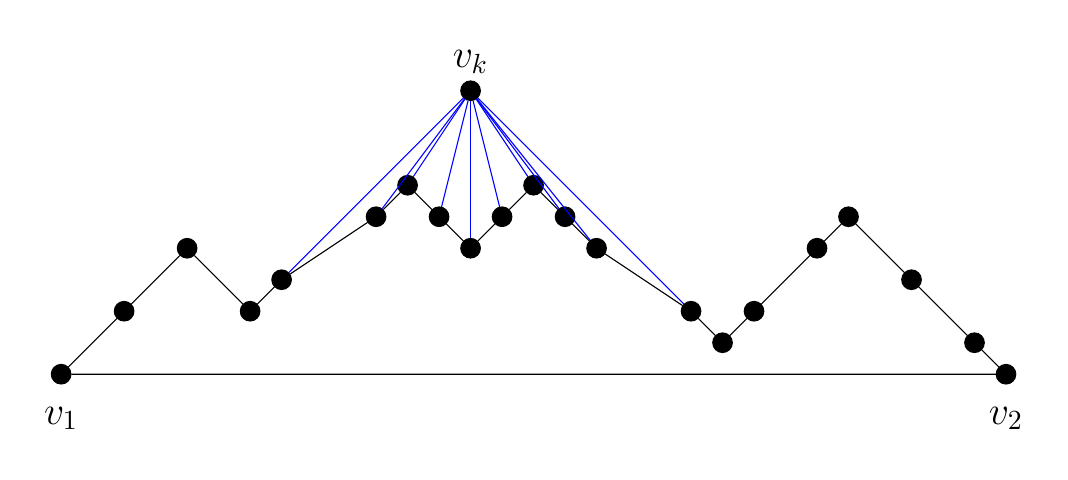
\begin{tikzpicture}[every node/.style={draw,circle,fill},node distance=0cm,scale=0.4]

%\draw[color=black!30](-1.5,-1.5)grid(30.5,10.5);

\foreach[count=\c] \x/\y in {0/0,2/2,4/4,6/2,7/3,
10/5,11/6,12/5,13/4,14/5,15/6,16/5,17/4,20/2,21/1,22/2,24/4,25/5,27/3,29/1,30/0}
	\node[scale=0.75] (v\c) at (\x,\y) {};

\draw (v1) -- (v2) -- (v3) -- (v4) -- (v5) -- (v6) -- (v7) -- (v8) -- (v9) -- (v10)--(v11) -- (v12) -- (v13) -- (v14) -- (v15) -- (v16) -- (v17) -- (v18) -- (v19) -- (v20) -- (v21)--(v1);

\node[draw=none,fill=none,below=of v1] {\Large$v_1$};
\node[draw=none,fill=none,below=of v21] {\Large$v_2$};

\node[scale=0.75] (vk) at (13,9) {};
\node[draw=none,fill=none,above=of vk,yshift=-0.2cm] {\Large$v_k$};

\foreach[count=\c] \x in {5,6,...,14}
	\draw[color=blue](vk)to(v\x);

\end{tikzpicture}};
\end{tikzpicture}
\topbreak
\vspace*{-2\baselineskip}
\subsubsection{Anmerkungen}
\begin{itemize}[itemsep=-1pt]
	\item für zwei Gitterpunkte mit \textit{Manhatten distance} ($L_1(P_1,P_2)=|x_1-x_2|+|y_1-y_2|$) wird der Gitterpunkt für $v_k$ durch den Schnittpunkt der Geraden mit Steigung $-1$ durch $P_2$ und Steigung $1$ durch $P_1$ berechnet (\algo{shift-Methode}{\begin{algorithm}[H]
	\SetAlgoVlined
	\SetKwProg{Fn}{Function}{}{end}
	\KwIn{triangulierter palanerer Graph $G=(V,E)$, kanonische Ordnung $\pi=(v_1,\dots,v_n)$}
	\KwData{Liste $L(v)$ mit allen Knoten, die mit dem Knoten $v$ verschoben werden müssen}
	\KwOut{planare, geradlinige Gitterzeichnung induziert durch die Koordinaten $P(v)=(x(v),y(v))$ für alle $v\in V$}
	\BlankLine
	\Begin{
		$P(v_1)=(0,0)$;\\
		$P(v_2)=(2,0)$;\\
		$P(v_3)=(1,1)$;\\
		$L(v_1)=\{v_i\}$ für $i=1,2,3$;\\
		\For{$k=4,\dots, n$}{
			$(w_1=v_1,w_2,\dots,w_{t-1},w_t=v_2)\leftarrow C_0(G_{k-1})$;\\
			$(w_p,\dots,w_q)\leftarrow$ Nachbarn von $v_k$ auf $C_0(G_{k-1})$;\\
			\ForAll{$v\in\bigcup\limits_{i=p+1}^{q-1} L(w_i)$}{
				$x(v)\leftarrow x(v)+1$\tcp*[r]{Verschiebung um $1$ nach rechts}
			}
			\ForAll{$v\in\bigcup\limits_{i=q}^{t} L(w_i)$}{
				$x(v)\leftarrow x(v)+2$\tcp*[r]{Verschiebung um $2$ nach rechts}
			}
			$P(v_k)\leftarrow\mu(P(w_p),P(w_q))$\tcp*[r]{$\mu(P_1,P_2)=(\frac{1}{2}(x_1-y_1+x_2+y_2),\frac{1}{2}(-x_1+y_1+x_2+y_2))$}
			$L(v_k)\leftarrow\{v_k\}\cup\bigcup\limits_{i=p+1}^{q-1}L(w_i)$;
		}
	}
\end{algorithm}})
	\item gestartet wird mit den Punkten $P(v_1)=(0,0),P(v_2)=(2,0),P(v_3)=(1,1)$ (entspricht $G_3$)
	\item Anfangslisten $L(v_i)=\{v_i\},i=1,2,3$
	\item zum Zeichnen von $G_k$ müssen folgende $3$ Invarianten gelten:
		\begin{enumerate}[itemsep=-1pt]
			\item $P(v_1)=(0,0)$ und $P(v_2)=(2k-4,0)$
			\item $x(w_1)<x(w_2)<\dots<x(w_t)$ für $C_0(G_k)=(v_1=w_1,\dots,w_t=v_2)$
			\item alle Kanten $(w_i,w_{i+1})$ auf $C_0(G_k)$ sind geradlinig mit Steigung $1$, bzw. $-1$
		\end{enumerate}
	\item Nachteil: sehr kleine Winkel möglich $\Rightarrow$ unleserliche Graphen können entstehen
\end{itemize}